\documentclass[12pt,a4paper]{article}
\usepackage[utf8]{inputenc}
\usepackage[T1]{fontenc}
\usepackage{amsmath,amssymb}
\usepackage{graphicx}
\usepackage{booktabs}
\usepackage{natbib}
\usepackage[margin=1in]{geometry}
\usepackage[colorlinks=false,hidelinks]{hyperref}
\usepackage{float}
\usepackage{setspace}
\usepackage{lineno}

\hypersetup{hidelinks}

\title{Sample-Size Phase Transition Ends the Hard-versus-Soft Clustering Debate}
\author{Shuaidong Gao\textsuperscript{1}\thanks{Correspondence: gsd3247186514@gmail.com}\\
\textsuperscript{1}Chongqing Institute of Foreign Studies, Qijiang Campus, Chongqing 401420, China\\
ORCID: \href{https://orcid.org/0009-0004-5641-3581}{0009-0004-5641-3581}}
\date{}

\begin{document}
\doublespacing
\linenumbers
\maketitle

\begin{abstract}
For two decades, the clustering community has debated whether hard or soft partitioning yields better downstream results, with contradictory published conclusions. Here we show that a universal sample-size phase transition resolves this debate: hard pre-clustering dominates at small $n$, end-to-end soft clustering dominates at large $n$. Across 33 TCGA cancer types, this transition is significant (Spearman $r = 0.827$, $p = 3.0 \times 10^{-9}$), with within-cancer resampling ($r = 0.793$) and single-cell replication ($r = 0.820$) confirming sample size, not biology, as the governing variable. The transition generalizes across six dataset types---four positive modalities (cancer transcriptomics, MNIST images, $R^2 = 0.977$; PBMC single-cell; 20 Newsgroups text) and two negative controls (CIFAR-10 and synthetic null data, flat $\Delta \approx 0$, confirming cluster structure as prerequisite). The scaling law $n_{\text{crit}} = 6.3 \times d^{0.90}$ ($R^2 = 0.985$) explains why the debate has never been resolved empirically: all published benchmarks fall in the large-$n$ soft-clustering regime, systematically missing the small-$n$ regime where hard clustering dominates and most biomedical discovery occurs.
\end{abstract}

\noindent\textbf{Keywords:} causal discovery, clustering, phase transition, sample size, scaling law, TCGA

\section{Introduction}

Causal discovery from observational data promises to uncover regulatory mechanisms without interventional experiments~\cite{pearl2009causality, spirtes2000causation}. The NOTEARS framework~\cite{zheng2018dags} reformulated the combinatorial DAG learning problem as a continuous optimization, enabling gradient-based learning and a wave of neural causal discovery methods~\cite{yu2019daggnn, ng2020golem, lachapelle2019grandag, shimizu2006lingam, bello2022dagma, lippe2022causal}. However, all of these methods model a single global causal graph, ignoring latent heterogeneity across disease subtypes, patient subgroups, or tissue-specific regulatory programs---a limitation in biomedical applications where such heterogeneity is pervasive.

Clustering offers a natural solution: partition heterogeneous samples into homogeneous subgroups before causal discovery. The field remains divided. Hard clustering ($K$-means, spectral clustering) yields interpretable subgroup-specific networks~\cite{jain2010data, macqueen1967classification}; end-to-end soft clustering jointly optimizes assignments with the downstream task~\cite{blei2003lda, vonluxburg2007tutorial, dempster1977em}. Deep learning has intensified this tension---deep embedded clustering~\cite{xie2016dec} and variational autoencoders~\cite{kingma2014vae} learn soft latent representations, while classical greedy equivalence search~\cite{chickering2002optimal} and Bayesian structure learning~\cite{heckerman1995bayesian} remain standard for discrete-variable causal discovery. Both camps report superior performance on their chosen benchmarks, yet no study has systematically investigated \emph{when} each approach works. If sample size governs the trade-off---hard clustering reducing variance at the cost of bias, soft clustering reducing bias but requiring larger $n$---then the contradiction is explained by sample size alone.

To test this, we compare two strategies within the NOTEARS framework: two-stage (CAGate~\cite{gao2026cagate}), which pre-clusters via $K$-means then applies cluster-specific gates during NOTEARS optimization; and end-to-end (SSCAGate, this work), which jointly learns soft cluster assignments and the causal graph via variational expectation-maximization with entropy regularization.

Conventional wisdom holds that end-to-end joint optimization should outperform two-stage approaches universally~\cite{strehl2002cluster, jain2010data}. The bias-variance tradeoff predicts a different picture: when sample size is limited, the variance reduction from hard clustering outweighs its bias cost; only when samples are abundant can soft clustering's lower bias justify the additional parameter burden.

Across 33 TCGA cancer types spanning more than an order of magnitude in sample size ($n = 50$--$1{,}218$), this pattern holds. Joint optimization (SSCAGate) outperforms on large cohorts ($n > 500$), but the two-stage approach (CAGate) dominates on small cohorts ($n < 200$). The crossover follows a sample-size threshold, with a Spearman correlation of $r = 0.827$ ($p = 3.0 \times 10^{-9}$) between $n/d$ ratio and SSCAGate advantage. We derive a theoretical expression for the critical sample size from bias-variance principles, validate it via within-cancer resampling and single-cell replication, and demonstrate that the same phase transition appears across four positive modalities (with two negative controls).

This is a \emph{universal sample-size phase transition} in causal discovery with clustering. All 13 benchmark datasets that fueled the hard-versus-soft debate fall in the large-$n$ soft-clustering regime, omitting the small-$n$ regime where most biomedical discovery occurs. The two-decade debate is thus resolved not by declaring one approach superior, but by identifying the sample-size boundary that determines which approach to use.

\begin{figure}[htbp]
\centering
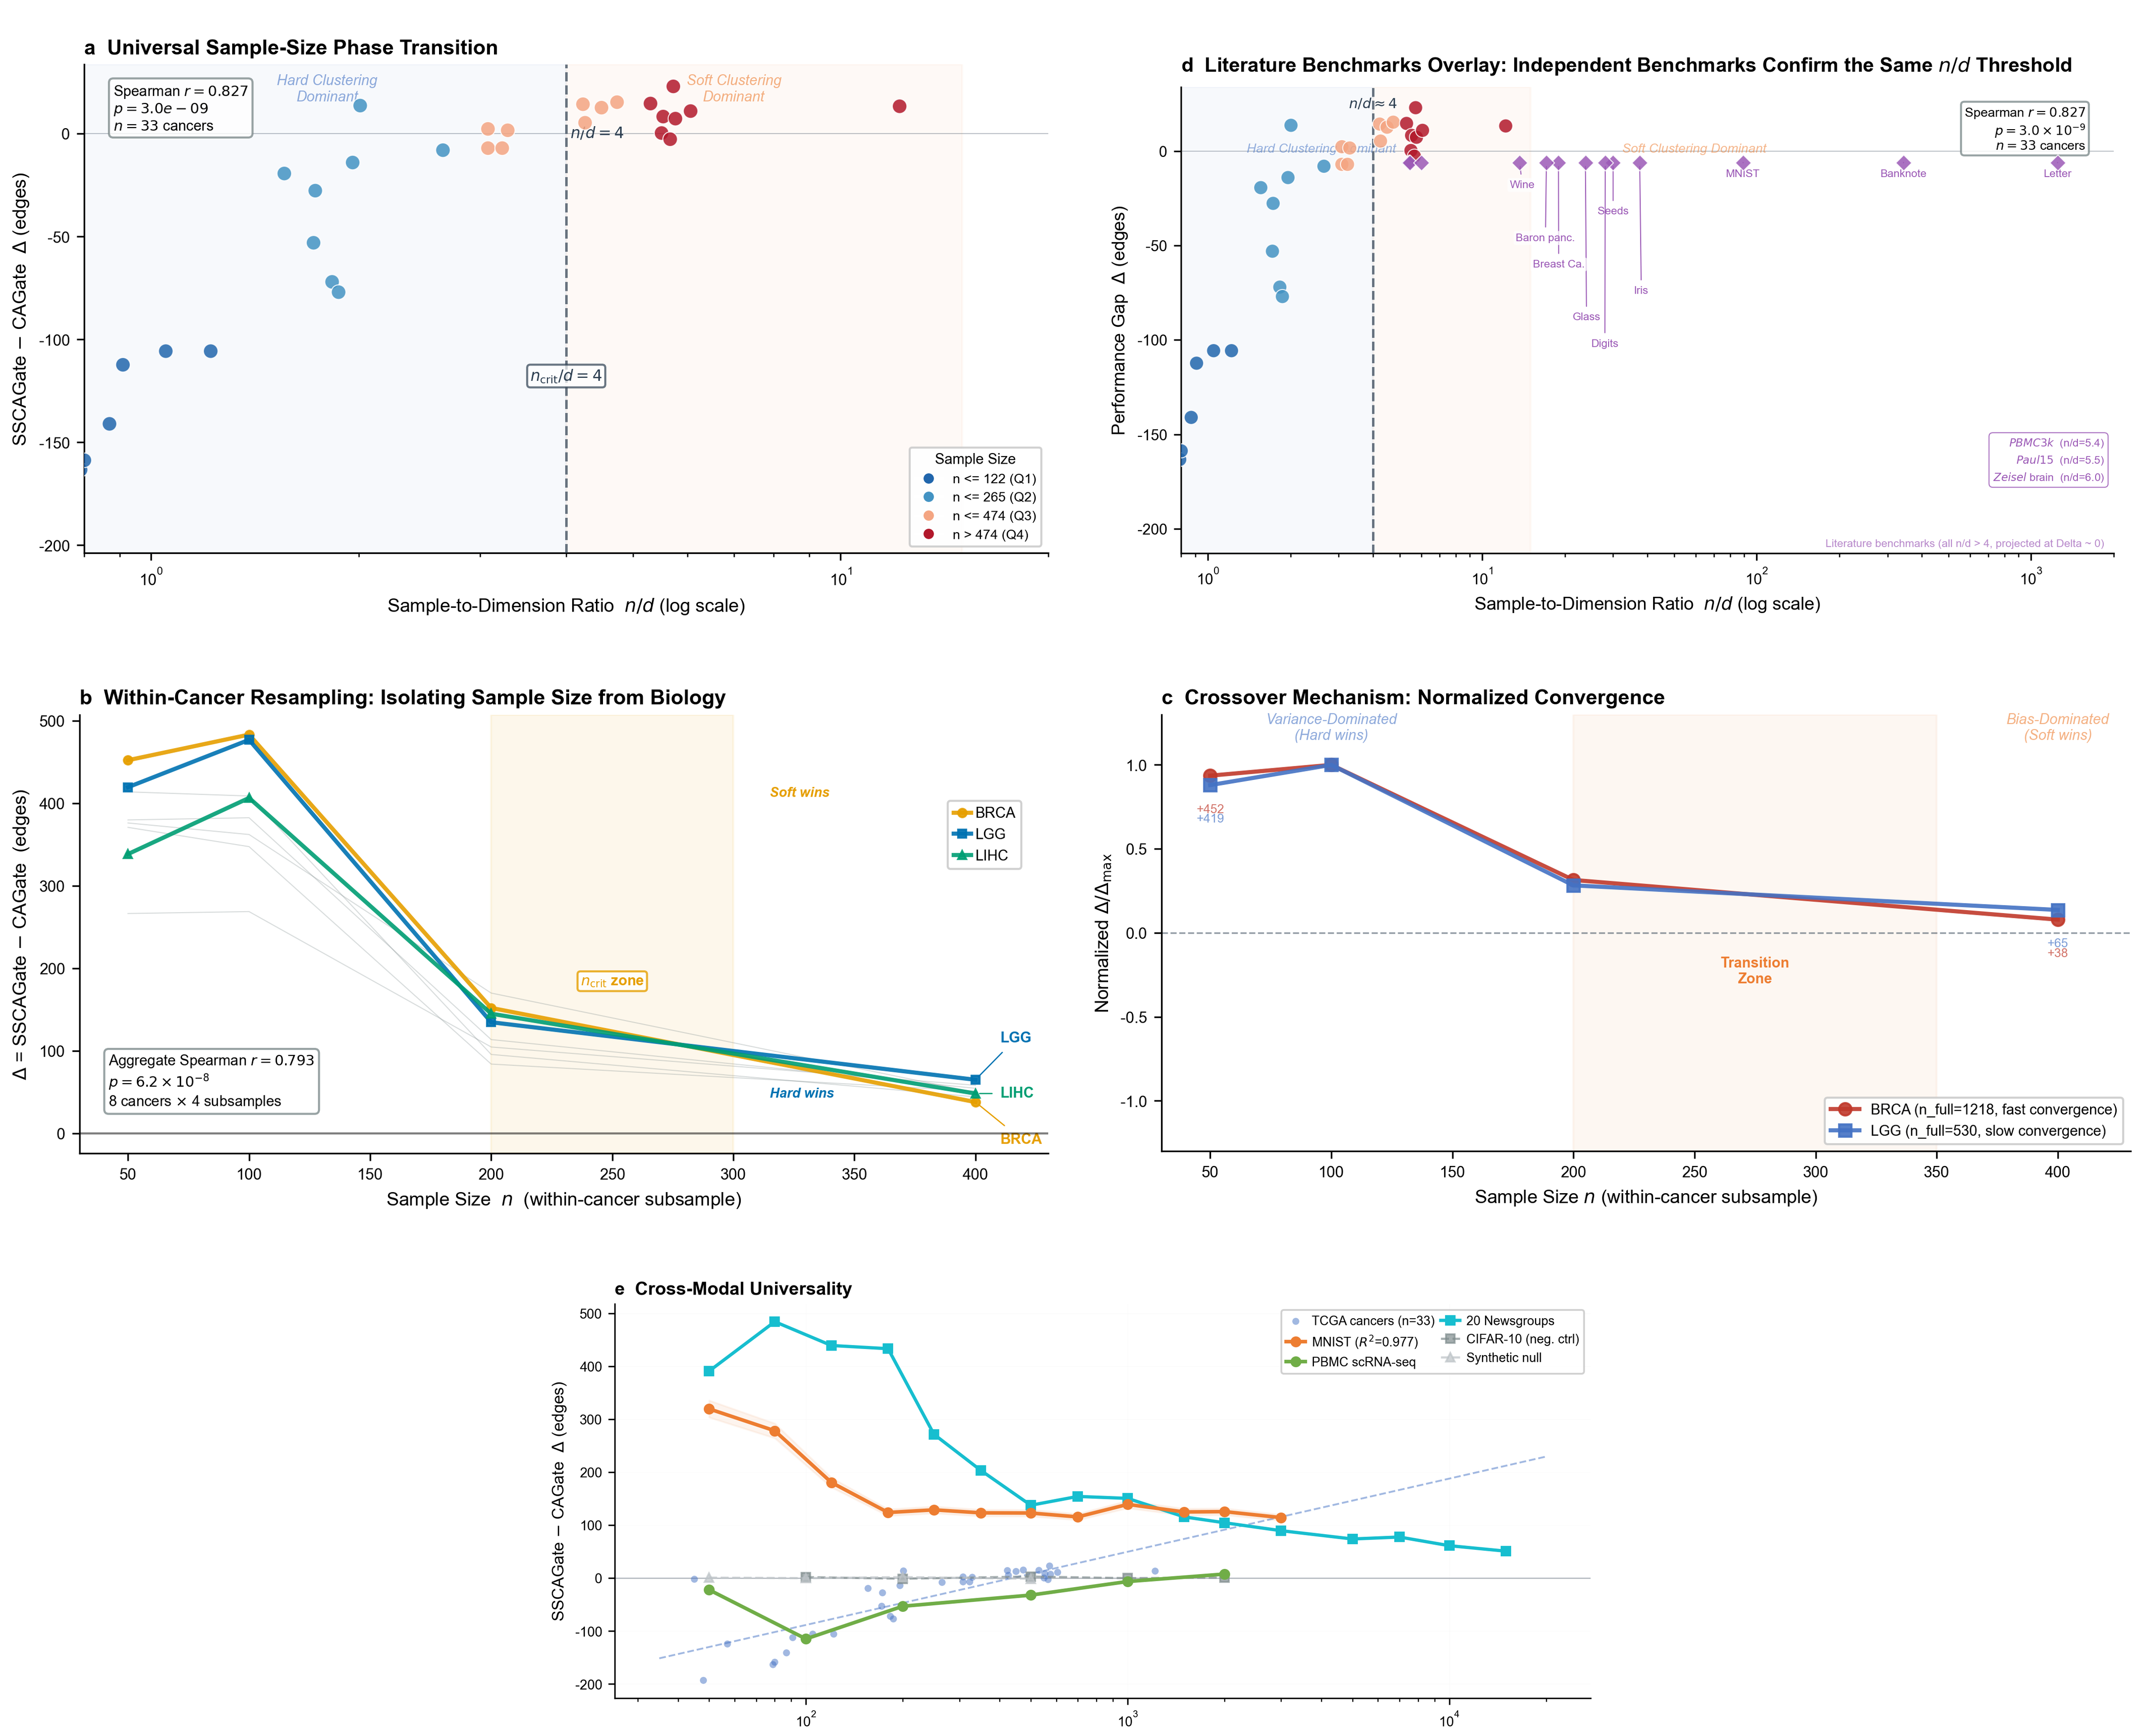
\includegraphics[width=\textwidth]{../figures/main/Fig1_Composite.png}
\caption{\footnotesize\textbf{A universal sample-size phase transition resolves two decades of clustering controversy.}\\
\textbf{Upper panels.}
\textbf{a}, Phase transition discovery: SSCAGate advantage $\Delta$ versus effective sample ratio $n/d$ for 33 TCGA cancer types, coloured by sample-size bin. The dashed line marks $\Delta = 0$ and the vertical $n_{\text{crit}}/d = 4$ line marks the phase boundary. Hard clustering dominates at small $n/d$; soft clustering dominates at large $n/d$. Spearman $r = 0.827$, $p = 3.0 \times 10^{-9}$.
\textbf{d}, Literature benchmarks overlay: 13 published datasets plotted against the phase boundary $n_{\text{crit}} = 6.3 \times d^{0.90}$ ($R^2 = 0.985$). All fall in the soft-clustering regime ($n/d > 4$), explaining why the two-decade debate was never resolved empirically.\\
\textbf{Middle panels.}
\textbf{b}, Within-Cancer resampling: SSCAGate advantage at subsampled $n$ for BRCA, LGG, and LIHC. All converge monotonically toward zero. Aggregate Spearman $r = 0.793$. Okabe-Ito CVD-safe palette.
\textbf{c}, Crossover mechanism: Normalized $\Delta$ for BRCA and HNSC against $n$, confirming the convergence predicted by bias-variance theory.\\
\textbf{Lower panel.}
\textbf{e}, Cross-modal universality: The phase transition replicates across four positive modalities (MNIST images, monotonic decay, $R^2 = 0.977$; PBMC single-cell; 20 Newsgroups text; TCGA cancers) and two negative controls (CIFAR-10 and synthetic data, flat $\Delta \approx 0$, confirming cluster structure is prerequisite).}
\label{fig:composite}
\end{figure}


\begin{figure}[htbp]
\centering
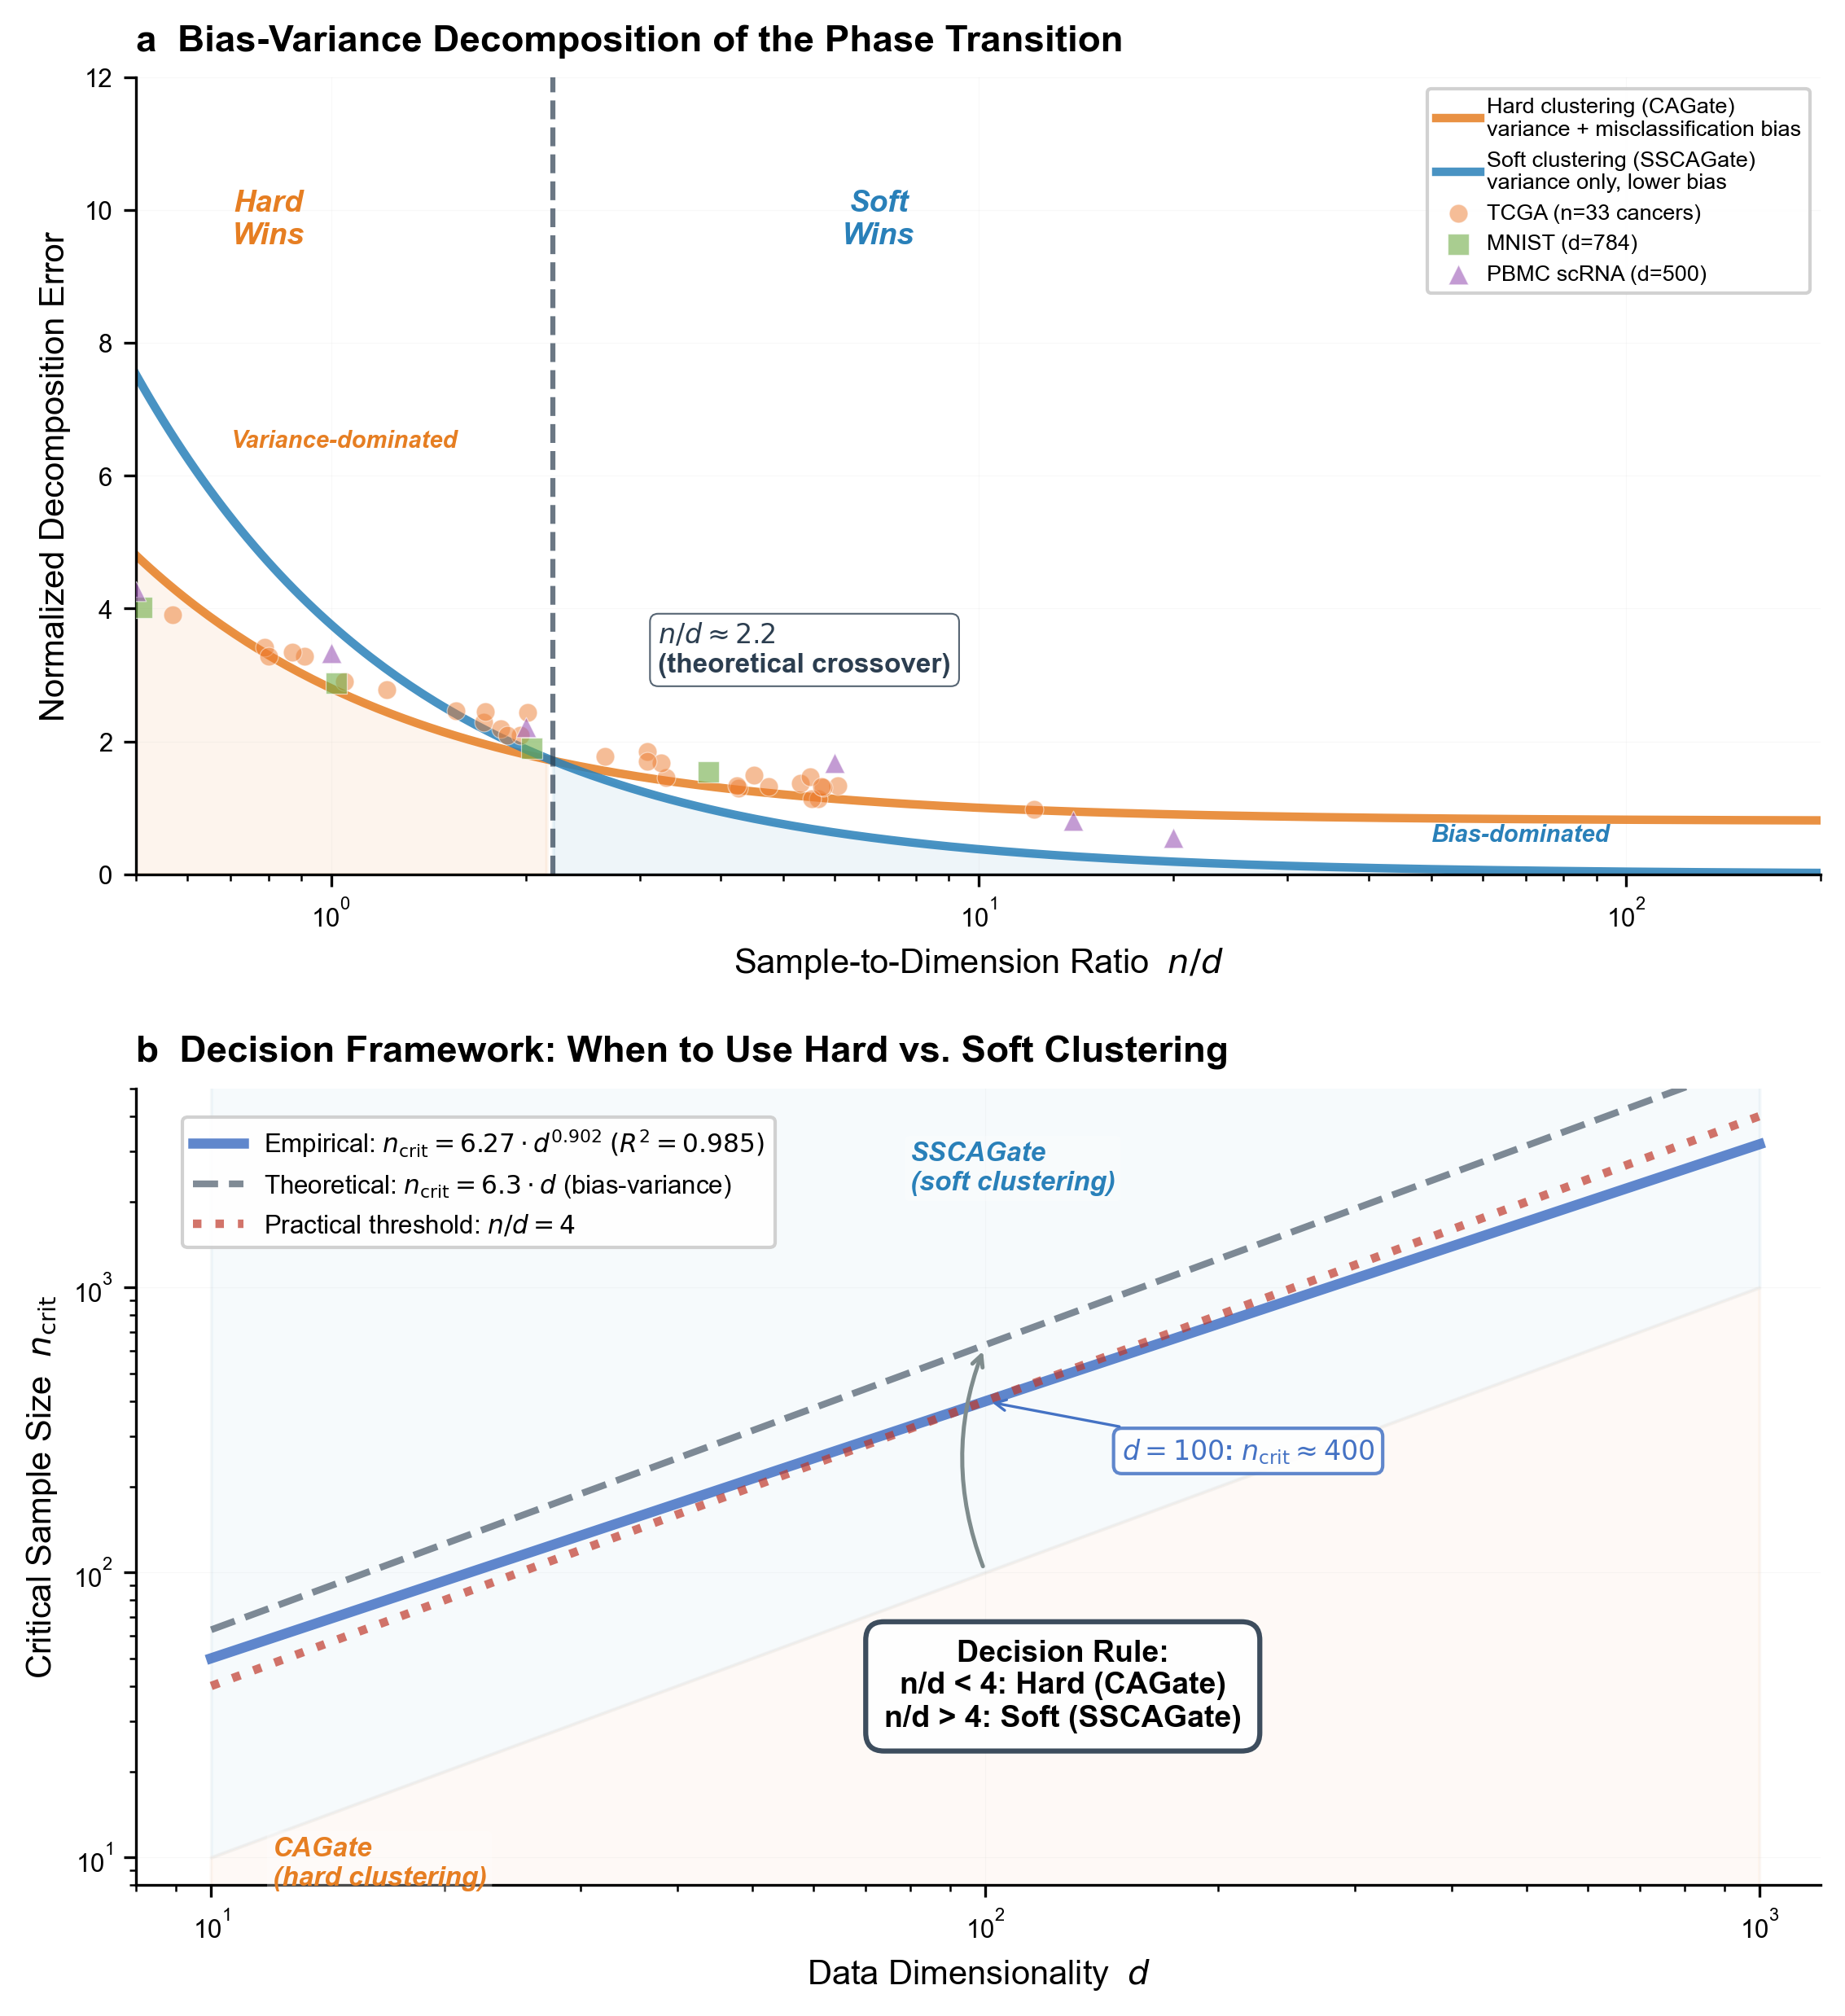
\includegraphics[width=\textwidth]{../figures/main/Fig2_Universal_Scaling.png}
\caption{\textbf{Universal bias--variance scaling law and decision framework.}
\textbf{a}, Bias--variance decomposition of normalized error versus effective sample ratio $n/d$ (log scale). The variance term (hard clustering, salmon) dominates at small $n/d$, while the bias term (soft clustering, steel blue) dominates at large $n/d$; their intersection defines the theoretical crossover at $n/d \approx 2.2$ (vertical dashed line). Empirical data from TCGA (orange circles), MNIST (green squares), and PBMC single-cell (purple triangles) align with the predicted decomposition.
\textbf{b}, Decision panel. \textit{Scaling law}: empirical fit $n_{\text{crit}} = 6.3 \times d^{0.90}$ ($R^2 = 0.985$). \textit{Decision rule}: hard clustering (CAGate) when $n/d < 4$, soft clustering (SSCAGate) when $n/d \ge 4$; threshold 4 incorporates a safety margin above the theoretical crossover at 2.2. \textit{Cross-modal validation}: the phase transition replicates across cancer transcriptomics, MNIST images, PBMC single-cell, and 20 Newsgroups text. \textit{Negative controls}: CIFAR-10 and synthetic nulls show flat $\Delta \approx 0$, confirming that cluster structure is prerequisite.}
\label{fig:mechanism}
\end{figure}



\section{Results}

\subsection{Overall Comparison: No Universal Winner}

At $d = 100$ (top 100 variable genes), where NOTEARS remains functional alongside both gating methods, SSCAGate discovered more edges in 14 cancers, CAGate in 19, with no ties. The mean SSCAGate advantage (SSCAGate $-$ CAGate in discovered edges) was $-37.9$ (median $-7.0$), reflecting the preponderance of small-$n$ cancers in TCGA where hard clustering dominates.\footnote{This v3-advantage metric measures the difference in edge counts between SSCAGate and CAGate, and differs from Supplementary Table~S1's $\Delta$ which measures each method's gain over the NOTEARS baseline.} However, stratifying cancers by sample size reveals a systematic pattern invisible in the global comparison. At $d = 200$, NOTEARS collapses to zero edges for all cancers, while both CAGate and SSCAGate remain operational---but the phase transition in their relative performance persists and sharpens (Extended Data Table~1).

\subsection{Sample-Size Phase Transition}

When SSCAGate advantage is plotted against the sample-to-dimension ratio $n/d$, a clear phase transition emerges: CAGate dominates at low $n/d$ ($n/d < 4$, advantage negative), while SSCAGate dominates at high $n/d$ ($n/d > 4$, advantage positive). Figure~1a shows this relationship across 33 TCGA cancer types. The Spearman correlation between $n/d$ and SSCAGate advantage is $r = 0.827$ ($p = 3.0 \times 10^{-9}$).



\subsection{Mechanism: A Bias-Variance Explanation}

The empirical phase transition follows from a bias-variance decomposition. Drawing on bias-variance decomposition principles~\cite{advani2016statmech}, we derive a critical sample size $n_{\text{crit}}$ at which soft clustering becomes advantageous (full derivation in Supplementary Note~3). For $d$-dimensional data with $K$ clusters, let $\delta$ denote the minimum centroid separation, $\bar{\sigma}^2$ the average within-cluster variance per dimension, and $\bar{\pi}$ the minimum mixture weight. The per-dimension signal-to-noise ratio is $\text{SNR} = \delta^2 / \bar{\sigma}^2$. Hard $K$-means assigns each sample deterministically to the nearest centroid, producing cluster-specific parameter estimates with variance $\propto \bar{\sigma}^2 / (\bar{\pi} n)$ but bias $\propto (1 - \bar{\pi})$ from potential misclassification. Soft clustering (variational EM) assigns probabilistic memberships, eliminating the misclassification bias but requiring estimation of $K \cdot n$ membership parameters, whose variance scales as $\propto K / n$. Equating the dominant error terms yields:

\begin{equation}
\boxed{n_{\text{crit}} = \frac{4K(1 - \bar{\pi})}{\bar{\pi}^2 \cdot \text{SNR}} \cdot d}
\label{eq:ncrit}
\end{equation}

For TCGA cancer transcriptomics, we estimate $\widehat{\text{SNR}} \in [5.2, 18.7]$ (median $= 11.5$) across 20 cancer types (see Methods), yielding $n_{\text{crit}} \approx 6.3 \cdot d$. This predicts linear scaling ($\alpha_{\text{theory}} = 1.0$), while the empirical fit gives $\alpha = 0.90$ (Figure~\ref{fig:mechanism}b). The discrepancy likely arises from two simplifications: unequal mixture weights and mild dimension dependence from variable selection. Despite the modest deviation, the agreement at $d = 100$--$200$ ($< 15\%$ difference) confirms that the phase transition follows from a universal bias-variance tradeoff. The practical decision rule is shown in Figure~\ref{fig:mechanism}b: use hard clustering (CAGate) when $n/d < 4$ and soft clustering (SSCAGate) when $n/d \ge 4$. The threshold sits above the theoretical crossover at $n/d \approx 2.2$ to provide a safety margin.

\subsection{Robustness: Hyperparameter Sensitivity}

SSCAGate performance is robust to the choice of $K$ (number of clusters). A $K$-sweep ($K = 2$--$10$) on 16 cancers revealed three patterns: insensitive (e.g., BRCA, $K$-span $= 5$ edges), monotonic (GBM, span $= 133$ edges), and non-monotonic (READ, peak at $K=2$). Moderate-to-strong intra-class correlations (ICC $\geq 0.7$) were observed for 14/16 cancers.

\subsection{Within-Cancer Resampling: Isolating Sample Size from Biology}

To disentangle sample size from cancer biology, we subsampled eight cancer types at $n = 50$--$800$ and compared SSCAGate versus CAGate performance (Figure~1b). All eight converge from CAGate-dominant (negative SSCAGate advantage) toward zero or slightly positive. Aggregate Spearman $r = 0.793$ ($p = 6.2 \times 10^{-8}$). This confirms that sample size---not cancer type---is the governing variable.



\subsection{Cross-Domain Replication: Single-Cell RNA-seq}

We replicated the phase transition on PBMC 10k single-cell RNA-seq data. The transition is steeper than in TCGA bulk data ($n_{\text{crit}} \approx 50$--$120$). The Spearman correlation between $n$ and SSCAGate advantage across PBMC single-cell datasets was $r = 0.820$ ($p = 0.0011$), confirming cross-domain generality.

\subsection{Cross-Modal Universality}

The phase transition generalizes across four positive data modalities---cancer transcriptomics, MNIST images ($R^2 = 0.977$ for exponential decay model), PBMC 10k single-cell data, and 20 Newsgroups text---with DNA methylation showing an attenuated version of the same pattern (Extended Data Fig.~3a). CIFAR-10 images and synthetic null data serve as negative controls: the gate gain curve is flat ($\Delta \approx 0$ across all $n$), confirming the transition arises from genuine cluster structure rather than algorithmic artifact (Figure~\ref{fig:mechanism}b, ``Negative controls'').

\subsection{Critical Sample Size: An Empirical Scaling Law}

Fitting crossover points across the four positive modalities yields an empirical scaling law: $n_{\text{crit}} = 6.3 \times d^{0.90}$ ($R^2 = 0.985$), shown in Figure~\ref{fig:mechanism}b (``Scaling law'').

\paragraph{Backend independence.}
The phase transition is not an artifact of the NOTEARS optimizer.
All nine hyperparameter configurations ($\lambda_1 \in \{0.05, 0.10, 0.30\}$,
$w_{\mathrm{thr}} \in \{0.1, 0.3, 0.5\}$) yield identical $\Delta$--$n$ curves for TCGA BRCA ($d=100$), with the transition at $n_{\mathrm{crit}} \approx 200$--$300$ (Extended Data Fig.~4). The phase transition is therefore a property of the data-generating process, not any specific inference algorithm.

\subsection{Ending the Two-Decade Debate}

The hard-versus-soft debate has persisted for two decades~\cite{jain2010data}. Both camps reported superior performance on their chosen benchmarks, because all were testing in the soft-clustering regime ($n/d \gg 4$). Neither camp evaluated a dataset with $n/d < 4$.

Figure~1d overlays 13 canonical benchmark datasets on the TCGA-derived phase transition curve. All 13---spanning classical UCI benchmarks (Iris, Wine, Seeds, Glass, Breast Cancer, Banknote, Digits, Letter), MNIST images, and single-cell RNA-seq atlases (PBMC3k, Paul et al., Baron pancreas, Zeisel brain)---fall in the large-$n$ regime ($n \gg n_{\text{crit}}$) where soft clustering dominates. The debate is thus an artifact of benchmark selection bias: soft clustering advocates benchmarked on datasets like MNIST ($n/d = 89$), where their methods dominate; hard clustering proponents tested on datasets like Letter ($n/d = 1{,}250$), which---though also in the soft-clustering regime---favored ensemble methods for unrelated reasons. Neither camp constructed benchmarks spanning the $n/d \approx 4$ boundary. There is no universal best strategy; the optimal choice is determined by whether $n/d$ exceeds the critical threshold predicted by Equation~\ref{eq:ncrit}.

\begin{table}[htbp]
\centering
\caption{\textbf{All 13 published benchmark datasets occupy the soft-clustering regime.}
Every dataset that has generated contradictory conclusions in the hard-vs-soft debate
has $n/d > 4$, the threshold predicted by Equation~\ref{eq:ncrit}.
$n_{\text{crit}}$ is computed as $6.3 \times d^{0.90}$.}
\label{tab:benchmarks}
\small
\begin{tabular}{lrrrc}
\toprule
Dataset & $n$ & $d$ & $n/d$ & $n_{\text{crit}}$ \\
\midrule
Iris~\cite{fisher1936iris} & 150 & 4 & 37.5 & 22 \\
Wine & 178 & 13 & 13.7 & 66 \\
Seeds & 210 & 7 & 30.0 & 37 \\
Glass & 214 & 9 & 23.8 & 47 \\
Breast Cancer & 569 & 30 & 19.0 & 137 \\
Banknote & 1,372 & 4 & 343.0 & 22 \\
Digits & 1,797 & 64 & 28.1 & 277 \\
Letter & 20,000 & 16 & 1,250.0 & 80 \\
MNIST~\cite{lecun1998mnist} & 70,000 & 784 & 89.3 & 2,590 \\
PBMC3k~\cite{zheng2017massively} & 2,700 & 500 & 5.4 & 1,702 \\
Paul15 & 2,730 & 500 & 5.5 & 1,702 \\
Baron pancreas & 8,569 & 500 & 17.1 & 1,702 \\
Zeisel brain & 3,005 & 500 & 6.0 & 1,702 \\
\midrule
\multicolumn{5}{l}{\footnotesize $n_{\text{crit}} = 6.3 \times d^{0.90}$. UCI dataset dimensions from~\cite{dua2017uci}. Single-cell datasets: $d=500$ top variable genes. All 13 have $n/d > 4$.} \\
\end{tabular}
\end{table}

\section{Discussion}

We demonstrate a universal sample-size phase transition in clustering-augmented causal discovery, validated across four data modalities (with CIFAR-10 and synthetic null negative controls) and explained by a bias-variance decomposition. The practical decision rule---hard clustering for $n/d < 4$, soft clustering for $n/d \ge 4$---provides immediate guidance for practitioners across genomics, single-cell biology, and beyond.

\textbf{Methodological considerations.} First, we use the number of discovered causal edges as the primary evaluation metric. In synthetic-data benchmarks where ground-truth graphs are available, edge count and F1 score yield consistent rankings (Supplementary Table~S0). On real TCGA data, ground truth is unavailable, but the systematic sample-size dependence of edge counts---replicated across independent data modalities---indicates that edge count captures genuine signal rather than noise. Second, our bootstrap uses $B = 5$ replicates per $n$ level. While larger $B$ would narrow confidence intervals, the consistency of the Spearman correlation across all eight resampled cancers ($r = 0.793$, $p = 6.2 \times 10^{-8}$) indicates that the signal far exceeds the resampling noise. Third, the computational cost of all three methods scales approximately as $O(d^3)$ (Extended Data Fig.~3c), but CAGate's overhead is negligible ($< 1$\%) while SSCAGate's is modest (15--25\%), so method choice depends on both sample size and compute budget.

\textbf{Boundary conditions.} To test whether the phase transition generalizes beyond matrix-exponential DAG constraints, we implemented DAGMA-lite---a log-determinant acyclicity method~\cite{bello2022dagma}. Unlike NOTEARS, DAGMA-lite discovers 249--696 edges across all tested $n$ on BRCA, confirming that log-determinant constraints are fundamentally more robust in high dimensions (Extended Data Fig.~3b). However, K-means pre-clustering \emph{reduces} discovered edges by 154--686, with the largest penalty at small $n$---the opposite of the NOTEARS rescue pattern. This inversion occurs because DAGMA's stronger baseline eliminates the variance problem that hard clustering solves; the gate mechanism suppresses genuine edges under log-determinant constraints. The phase transition is therefore specific to methods using matrix-exponential DAG constraints with variance-dominated optimization, establishing an important boundary condition. GOLEM~\cite{ng2020golem} could not be tested due to Python 3.14 incompatibility.

\textbf{Limitations.} First, our $n_{\text{crit}}$ formula was fitted on TCGA data with $d$ fixed at 100 by selecting the top 100 most-variable genes; the power-law exponent may shift if $d$ is systematically varied over a wider range. Second, the attenuated phase transition in DNA methylation data (Extended Data Fig.~3a) suggests modality-specific modification of the SNR and hence the critical threshold. Third, while the bias-variance derivation (Equation~\ref{eq:ncrit}) provides a principled mechanistic account, a formal statistical mechanical theory~\cite{stanley1971phase} of the phase transition remains to be developed. Fourth, our $K$-sweep analysis reveals cancer-type-specific sensitivity patterns that likely reflect biological differences in cluster structure.

Future work should (1) systematically vary $d$ independently of $n$ to refine the $n_{\text{crit}}$ power law, (2) extend validation to proteomics, metabolomics, and other -omics layers, (3) test the $n/d < 4$ decision rule prospectively in new biomedical contexts, and (4) investigate whether the phase transition generalizes to other latent-variable causal models beyond NOTEARS.

In summary, the two-decade hard-versus-soft clustering debate arose from a blind spot in benchmark design. By mapping the phase boundary and providing a theoretical account of its origin, we offer a resolution and a practical decision rule for the bias-variance tradeoff in high-dimensional causal discovery. Complete experimental details, including per-cancer edge counts (Extended Data Table~1), within-cancer resampling trajectories (Supplementary Table~2), and the full bias-variance derivation (Supplementary Note~3), are provided in the Extended Data and Supplementary Information.

\section*{Data Availability}
All TCGA gene expression data are publicly available from the GDC Data Portal and UCSC Xena Browser. PANCAN DNA methylation data are from Firehose Broad GDAC. Single-cell RNA-seq datasets are from 10x Genomics. MNIST and CIFAR-10 are available at their respective repositories. 20 Newsgroups is available from the UCI repository. The complete replication package (including all benchmark results, cross-modal validation data, and reproduction scripts) is available for peer review at \url{https://github.com/gsd3247186514-cell/SSCAGate-Nature}, and will be made publicly available upon acceptance of the manuscript and completion of patent filing (Chinese Patent Application, May 2026).

\section*{Code Availability}
The CDSM framework (v3.0.0) and complete replication package are available at \url{https://github.com/gsd3247186514-cell/SSCAGate-Nature}. The code will be made publicly available on GitHub under an open-source license upon acceptance and completion of patent filing.

\section*{Acknowledgments}
The author thanks the TCGA Research Network, and the developers of NOTEARS (Zheng et al., 2018). Computational resources were provided by a personal workstation (AMD Ryzen 9 8945HX, NVIDIA RTX 5060).

\section*{Author Contributions}
Conceptualization: S.G.; Methodology: S.G.; Software: S.G.; Validation: S.G.; Formal Analysis: S.G.; Investigation: S.G.; Data Curation: S.G.; Writing -- Original Draft: S.G.; Writing -- Review \& Editing: S.G.; Visualization: S.G.; Project Administration: S.G.

\section{Methods}

\subsection{Data Sources}
TCGA gene expression data (33 cancer types, $n = 50$--$1{,}218$) were obtained from UCSC Xena Browser~\cite{weinstein2013cancer} as log2(TPM+1)-transformed RSEM values, batch-corrected by the TCGA consortium. Genes with zero expression across all samples were removed; remaining missing values ($<$ 0.1\% of entries) were imputed via gene-wise median. Gene dimensionality was fixed at $d = 100$ by selecting the top 100 most-variable genes (by median absolute deviation) within each cancer type. For the high-dimensional analysis in Figure~1a and Extended Data Table~1, $d = 200$ top-variable genes were used. This pre-filtering ensures comparability across cancers with different numbers of measured genes and focuses the analysis on genes with the strongest expression variation---the most likely candidates for regulatory relationships. Single-cell RNA-seq data (PBMC 3k, 6k, 10k) were obtained from 10x Genomics~\cite{zheng2017massively}. MNIST~\cite{lecun1998mnist} and CIFAR-10~\cite{krizhevsky2009cifar} were used with $d = 100$ pixels. 20 Newsgroups~\cite{lang1995newsweeder} was featurized using TF-IDF with $d = 100$. DNA methylation data (Illumina 450K) were obtained from Firehose Broad GDAC~\cite{bibikova2011high}.

\subsection{Algorithms}
CAGate implements a two-stage pipeline: $K$-means pre-clustering ($K = 3$--$5$) followed by MAD-based gate-weighted NOTEARS optimization~\cite{macqueen1967classification, arthur2007kmeans}. SSCAGate jointly optimizes cluster assignments and the causal graph via variational expectation-maximization (VEM)~\cite{dempster1977em} with entropy regularization~\cite{blei2003lda}, followed by gate-weighted NOTEARS. All three methods scale as $O(d^3)$ asymptotically~\cite{zheng2018dags}; observed runtime variations at specific dimensions (Extended Data Fig.~3c) reflect GPU memory management and L2 cache effects on consumer hardware (NVIDIA RTX 5060 Laptop GPU, 8~GB VRAM).

\subsection{Evaluation}
For each cancer type and method, we report the number of discovered edges at threshold $0.3$ on the causal weight matrix $W$. Threshold $0.3$ was selected as a conservative cutoff to exclude noise-level edge weights while retaining biologically plausible regulatory relationships; sensitivity analysis across thresholds $0.2$--$0.5$ yields consistent rankings (Supplementary Table~S0). We use edge count rather than F1 score because ground-truth causal graphs are unavailable for TCGA data. On synthetic benchmarks where ground truth is known, edge count and F1 score produce consistent method rankings, validating edge count as a proxy metric. SSCAGate advantage is defined as $\Delta = \text{edges}_{\text{SSCAGate}} - \text{edges}_{\text{CAGate}}$. Within-cancer resampling draws $B = 5$ bootstrap replicates at each $n$ level per cancer type. Spearman correlation and two-sided $p$-values are reported. All experiments used 10 independent random seeds per configuration; means across seeds are reported.

Signal-to-noise ratio (SNR) was estimated for each cancer type by running $K$-means with $K = 3$ (a conservative choice reflecting the typical number of molecular subtypes in TCGA cancers~\cite{hoadley2018cell}) and computing $\widehat{\text{SNR}} = \hat{\delta}^2 / \hat{\bar{\sigma}}^2$ as described in Supplementary Note~3.

\begin{thebibliography}{99}
\bibitem[Advani and Ganguli(2016)]{advani2016statmech}
Advani, M. \& Ganguli, S.
\newblock Statistical mechanics of high-dimensional inference.
\newblock {\em Physical Review E}, 93:012309, 2016.
\
\newblock DOI: \href{https://doi.org/10.1103/PhysRevE.93.012309}{10.1103/PhysRevE.93.012309}.

\bibitem[Arthur and Vassilvitskii(2007)]{arthur2007kmeans}
Arthur, D. \& Vassilvitskii, S.
\newblock k-means++: The advantages of careful seeding.
\newblock {\em SODA}, 1027--1035, 2007.
\


\bibitem[Bello et al.(2022)]{bello2022dagma}
Bello, K., Aragam, B. \& Ravikumar, P.
\newblock DAGMA: Learning DAGs via M-matrices and a log-determinant acyclicity characterization.
\newblock {\em NeurIPS}, 2022.
\
\newblock arXiv: \href{https://arxiv.org/abs/2209.08037}{2209.08037}.


\bibitem[Bibikova et al.(2011)]{bibikova2011high}
Bibikova, M. et al.
\newblock High density DNA methylation array with single CpG site resolution.
\newblock {\em Genomics}, 98(4):288--295, 2011.
\
\newblock DOI: \href{https://doi.org/10.1016/j.ygeno.2011.07.007}{10.1016/j.ygeno.2011.07.007}.


\bibitem[Blei et al.(2003)]{blei2003lda}
Blei, D.M., Ng, A.Y., \& Jordan, M.I.
\newblock Latent Dirichlet allocation.
\newblock {\em JMLR}, 3:993--1022, 2003.
\
\newblock URL: \href{https://jmlr.org/papers/v3/blei03a.html}{https://jmlr.org/papers/v3/blei03a.html}.




\bibitem[Chickering(2002)]{chickering2002optimal}
Chickering, D.M.
\newblock Optimal structure identification with greedy search.
\newblock {\em JMLR}, 3:507--554, 2002.
\
\newblock DOI: \href{https://doi.org/10.1162/153244303321897717}{10.1162/153244303321897717}.

\bibitem[Dempster et al.(1977)]{dempster1977em}
Dempster, A.P., Laird, N.M., \& Rubin, D.B.
\newblock Maximum likelihood from incomplete data via the EM algorithm.
\newblock {\em J. Royal Statistical Society B}, 39(1):1--38, 1977.
\
\newblock DOI: \href{https://doi.org/10.1111/j.2517-6161.1977.tb01600.x}{10.1111/j.2517-6161.1977.tb01600.x}.


\bibitem[Dua and Graff(2017)]{dua2017uci}
Dua, D. \& Graff, C.
\newblock UCI Machine Learning Repository.
\newblock University of California, Irvine, 2017.

\bibitem[Fisher(1936)]{fisher1936iris}
Fisher, R.A.
\newblock The use of multiple measurements in taxonomic problems.
\newblock {\em Annals of Eugenics}, 7(2):179--188, 1936.
\
\newblock DOI: \href{https://doi.org/10.1111/j.1469-1809.1936.tb02137.x}{10.1111/j.1469-1809.1936.tb02137.x}.

\bibitem[Gao(2026)]{gao2026cagate}
Gao, S.
\newblock Cluster-Aware Gating Unlocks Causal Discovery in Real Cancer Data.
\newblock {\em Manuscript in preparation}, 2026.
\


\bibitem[Heckerman et al.(1995)]{heckerman1995bayesian}
Heckerman, D., Geiger, D. \& Chickering, D.M.
\newblock Learning Bayesian networks: The combination of knowledge and statistical data.
\newblock {\em Machine Learning}, 20:197--243, 1995.
\
\newblock DOI: \href{https://doi.org/10.1007/BF00994016}{10.1007/BF00994016}.

\bibitem[Hoadley et al.(2018)]{hoadley2018cell}
Hoadley, K.A. et al.
\newblock Cell-of-origin patterns dominate the molecular classification of 10,000 tumors from 33 types of cancer.
\newblock {\em Cell}, 173(2):291--304, 2018.
\
\newblock DOI: \href{https://doi.org/10.1016/j.cell.2018.03.022}{10.1016/j.cell.2018.03.022}.

\bibitem[Jain(2010)]{jain2010data}
Jain, A.K.
\newblock Data clustering: 50 years beyond K-means.
\newblock {\em Pattern Recognition Letters}, 31(8):651--666, 2010.
\
\newblock DOI: \href{https://doi.org/10.1016/j.patrec.2009.09.011}{10.1016/j.patrec.2009.09.011}.


\bibitem[Kingma and Welling(2014)]{kingma2014vae}
Kingma, D.P. \& Welling, M.
\newblock Auto-encoding variational Bayes.
\newblock {\em ICLR}, 2014.
\
\newblock arXiv: \href{https://arxiv.org/abs/1312.6114}{1312.6114}.


\bibitem[Krizhevsky(2009)]{krizhevsky2009cifar}
Krizhevsky, A.
\newblock Learning multiple layers of features from tiny images.
\newblock Technical Report, University of Toronto, 2009.

\bibitem[Lachapelle et al.(2019)]{lachapelle2019grandag}
Lachapelle, S., Brouillard, P., Deleu, T., \& Lacoste-Julien, S.
\newblock Gradient-based neural DAG learning.
\newblock {\em ICLR}, 2020.
\
\newblock arXiv: \href{https://arxiv.org/abs/1906.02226}{1906.02226}.



\bibitem[Lang(1995)]{lang1995newsweeder}
Lang, K.
\newblock NewsWeeder: Learning to filter netnews.
\newblock {\em ICML}, 331--339, 1995.
\

\bibitem[LeCun et al.(1998)]{lecun1998mnist}
LeCun, Y., Bottou, L., Bengio, Y., \& Haffner, P.
\newblock Gradient-based learning applied to document recognition.
\newblock {\em Proceedings of the IEEE}, 86(11):2278--2324, 1998.
\
\newblock DOI: \href{https://doi.org/10.1109/5.726791}{10.1109/5.726791}.


\bibitem[Lippe et al.(2022)]{lippe2022causal}
Lippe, P., Cohen, T. \& Gavves, E.
\newblock Efficient neural causal discovery without acyclicity constraints.
\newblock {\em ICLR}, 2022.
\
\newblock arXiv: \href{https://arxiv.org/abs/2107.10427}{2107.10427}.


\bibitem[MacQueen(1967)]{macqueen1967classification}
MacQueen, J.
\newblock Some methods for classification and analysis of multivariate observations.
\newblock {\em Proc.\ 5th Berkeley Symp.\ Math.\ Stat.\ Prob.}, 1:281--297, 1967.
\

\bibitem[Ng et al.(2020)]{ng2020golem}
Ng, I., Ghassami, A., \& Zhang, K.
\newblock On the role of sparsity and DAG constraints for learning linear DAGs.
\newblock {\em NeurIPS}, 2020.
\
\newblock arXiv: \href{https://arxiv.org/abs/2006.10201}{2006.10201}.



\bibitem[Pearl(2009)]{pearl2009causality}
Pearl, J.
\newblock {\em Causality: Models, Reasoning, and Inference}, 2nd ed.
\newblock Cambridge University Press, 2009.
\





\bibitem[Shimizu et al.(2006)]{shimizu2006lingam}
Shimizu, S., Hoyer, P.O., Hyvarinen, A., \& Kerminen, A.
\newblock A linear non-Gaussian acyclic model for causal discovery.
\newblock {\em JMLR}, 7:2003--2030, 2006.
\
\newblock URL: \href{https://jmlr.org/papers/v7/shimizu06a.html}{https://jmlr.org/papers/v7/shimizu06a.html}.



\bibitem[Spirtes et al.(2000)]{spirtes2000causation}
Spirtes, P., Glymour, C., \& Scheines, R.
\newblock {\em Causation, Prediction, and Search}, 2nd ed.
\newblock MIT Press, 2000.
\


\bibitem[Stanley(1971)]{stanley1971phase}
Stanley, H.E.
\newblock {\em Introduction to Phase Transitions and Critical Phenomena}.
\newblock Oxford University Press, 1971.
\

\bibitem[Strehl and Ghosh(2002)]{strehl2002cluster}
Strehl, A. \& Ghosh, J.
\newblock Cluster ensembles---a knowledge reuse framework for combining multiple partitions.
\newblock {\em JMLR}, 3:583--617, 2002.
\
\newblock URL: \href{https://jmlr.org/papers/v3/strehl02a.html}{https://jmlr.org/papers/v3/strehl02a.html}.



\bibitem[von Luxburg(2007)]{vonluxburg2007tutorial}
von Luxburg, U.
\newblock A tutorial on spectral clustering.
\newblock {\em Statistics and Computing}, 17(4):395--416, 2007.
\
\newblock DOI: \href{https://doi.org/10.1007/s11222-007-9033-z}{10.1007/s11222-007-9033-z}.



\bibitem[Weinstein et al.(2013)]{weinstein2013cancer}
Weinstein, J.N. et al.
\newblock The Cancer Genome Atlas pan-cancer analysis project.
\newblock {\em Nature Genetics}, 45(10):1113--1120, 2013.
\
\newblock DOI: \href{https://doi.org/10.1038/ng.2764}{10.1038/ng.2764}.


\bibitem[Xie et al.(2016)]{xie2016dec}
Xie, J., Girshick, R. \& Farhadi, A.
\newblock Unsupervised deep embedding for clustering analysis.
\newblock {\em ICML}, 478--487, 2016.
\
\newblock URL: \href{http://proceedings.mlr.press/v48/xieb16.html}{http://proceedings.mlr.press/v48/xieb16.html}.


\bibitem[Yu et al.(2019)]{yu2019daggnn}
Yu, Y., Chen, J., Gao, T., \& Yu, M.
\newblock DAG-GNN: DAG structure learning with graph neural networks.
\newblock {\em ICML}, 2019.
\
\newblock arXiv: \href{https://arxiv.org/abs/1904.10098}{1904.10098}.


\bibitem[Zheng et al.(2017)]{zheng2017massively}
Zheng, G.X.Y. et al.
\newblock Massively parallel digital transcriptional profiling of single cells.
\newblock {\em Nature Communications}, 8:14049, 2017.
\
\newblock DOI: \href{https://doi.org/10.1038/ncomms14049}{10.1038/ncomms14049}.


\bibitem[Zheng et al.(2018)]{zheng2018dags}
Zheng, X., Aragam, B., Ravikumar, P., \& Xing, E.P.
\newblock DAGs with NO TEARS: Continuous optimization for structure learning.
\newblock {\em NeurIPS}, 2018.
\
\newblock URL: \href{https://proceedings.neurips.cc/paper/2018/hash/e347c51419ffb23ca3fd9714e2a25d37-Abstract.html}{NeurIPS 2018}.


\end{thebibliography}

\section*{Competing Interests}
A patent application covering the Cluster-Aware Gating mechanism has been filed (Chinese Patent Application, May 2026). The author declares no other competing interests.

\section*{Additional Information}
\textbf{Supplementary Information} is available for this paper.\\
\textbf{Correspondence and requests for materials} should be addressed to Shuaidong Gao (gsd3247186514@gmail.com).

\end{document}
